\section{Introduction}

\section{Background}

\section{Experimental}
CdTe films were deposited on both the as-received and
reconstructed surface of (100) SrTiO3 (MTI Corporation). Step-
terrace formation relied upon the miscut originating from the
inaccuracies in the crystallographic alignment carried out prior to
the cutting and polishing of the substrates (manufacturer’s miscut
tolerance 0.58). As a result, the degree of miscut could only be
varied through the use of substrates from different batches. Due to
the high temperatures required, the surface reconstruction took
place ex situ in a quartz tube furnace. Prior to annealing, the
substrates were etched in BHF for 90 s. Anneals were conducted in
flowing oxygen (60 cm3/min) at 1000 8C for 10 h. \cref{fig:srtio3_sub_afm} shows
atomic force microscopy (AFM) images for the as-received and
surface reconstructed substrates relevant to this work. As
expected, only the annealed substrates exhibit the step-terrace
structure with unit cell step heights. The difference in terrace
width for the surfaces shown in \cref{fig:srtio3_sub_afm}b and c can be attributed to a
miscut difference estimated at 0.358. Also present on each image
are the crystallographic axes obtained through X-ray diffraction
(XRD). Note that a nearly identical in-plane step direction exists for
both reconstructed surfaces. As this direction is close to, but not
aligned with the [0 1 1] axis of SrTiO3, it is expected that the steps
exhibit a saw-tooth morphology, but on length scales not readily
observed using atomic force microscopy.
\begin{figure}
    \centering
    \missingfigure{SrTio3 AFM Image}
    \caption{\label{fig:srtio3_sub_afm}AFM images for the (a) as-received (1 0 0) SrTiO3 substrate, (b) a reconstructed surface with an average terrace width of approximately 200 nm and (c) a reconstructed
        surface with a terrace width of approximately 50 nm. From the step heights and terrace widths it is estimated that the miscuts for the two reconstructed surfaces are (b) 0.118\degree
        and (c) 0.468\degree.}
\end{figure}

CdTe films were deposited on the three SrTiO3 surfaces shown
in \cref{fig:srtio3_sub_afm} using pulsed laser deposition. A deposition rate of 20 nm/min was achieved by
operating the laser at a repetition rate of 10 Hz with a substrate to
target distance of 3.5 cm. Films were grown to
a thickness of 300 nm as determined using a spectroscopic variable
angle ellipsometer (Horiba Jobin Yvon, France). Morphological and
structural characterization was then conducted on the films
produced using AFM and 2DXRD.
\section{Results and Discussion}
\cref{fig:srtio3_pole} shows the (1 1 1) CdTe pole figures for the three substrates
shown in \cref{fig:srtio3_sub_afm}. The dramatic differences observed between films
deposited on the as-received and annealed substrates indicate that
the surface reconstruction gives rise to a complete re-alignment of
the CdTe grains. The pole figure for the as-received surface is
consistent with a [1 1 1] oriented film. The fact that twelve peaks
exist in the outer ring, instead of the three expected for a single
crystal, indicates that there are four in-plane grain orientations.
The pole figures for the films deposited on the surface reconstructed substrates show that both films are predominantly [2 1 1]
oriented. The twelve peaks in the central ring and twenty-four
peaks in the outer ring denote twelve in-plane grain orientations. Each peak in the central ring comes from a different grain, the intensity differences indicate that some grains form
preferentially over others. Note that of the twelve peaks both
the strongest and weakest is in-line with the miscut direction for
both of the reconstructed surfaces and that the degree of this
preferential orientation is stronger for the reconstructed surface
having the narrow terrace width. An examination of the low
intensity pole figure peaks (not visible in the figures), indicates that
some [1 1 1] CdTe grains exist in these nominally [2 1 1] films, but
at the 10\% level. While these [1 1 1] grains contribute to
the intensity at the center of the pole, the response there is almost
entirely due to the (1 0 0) SrTiO3 substrate.
\begin{figure}
    \centering
    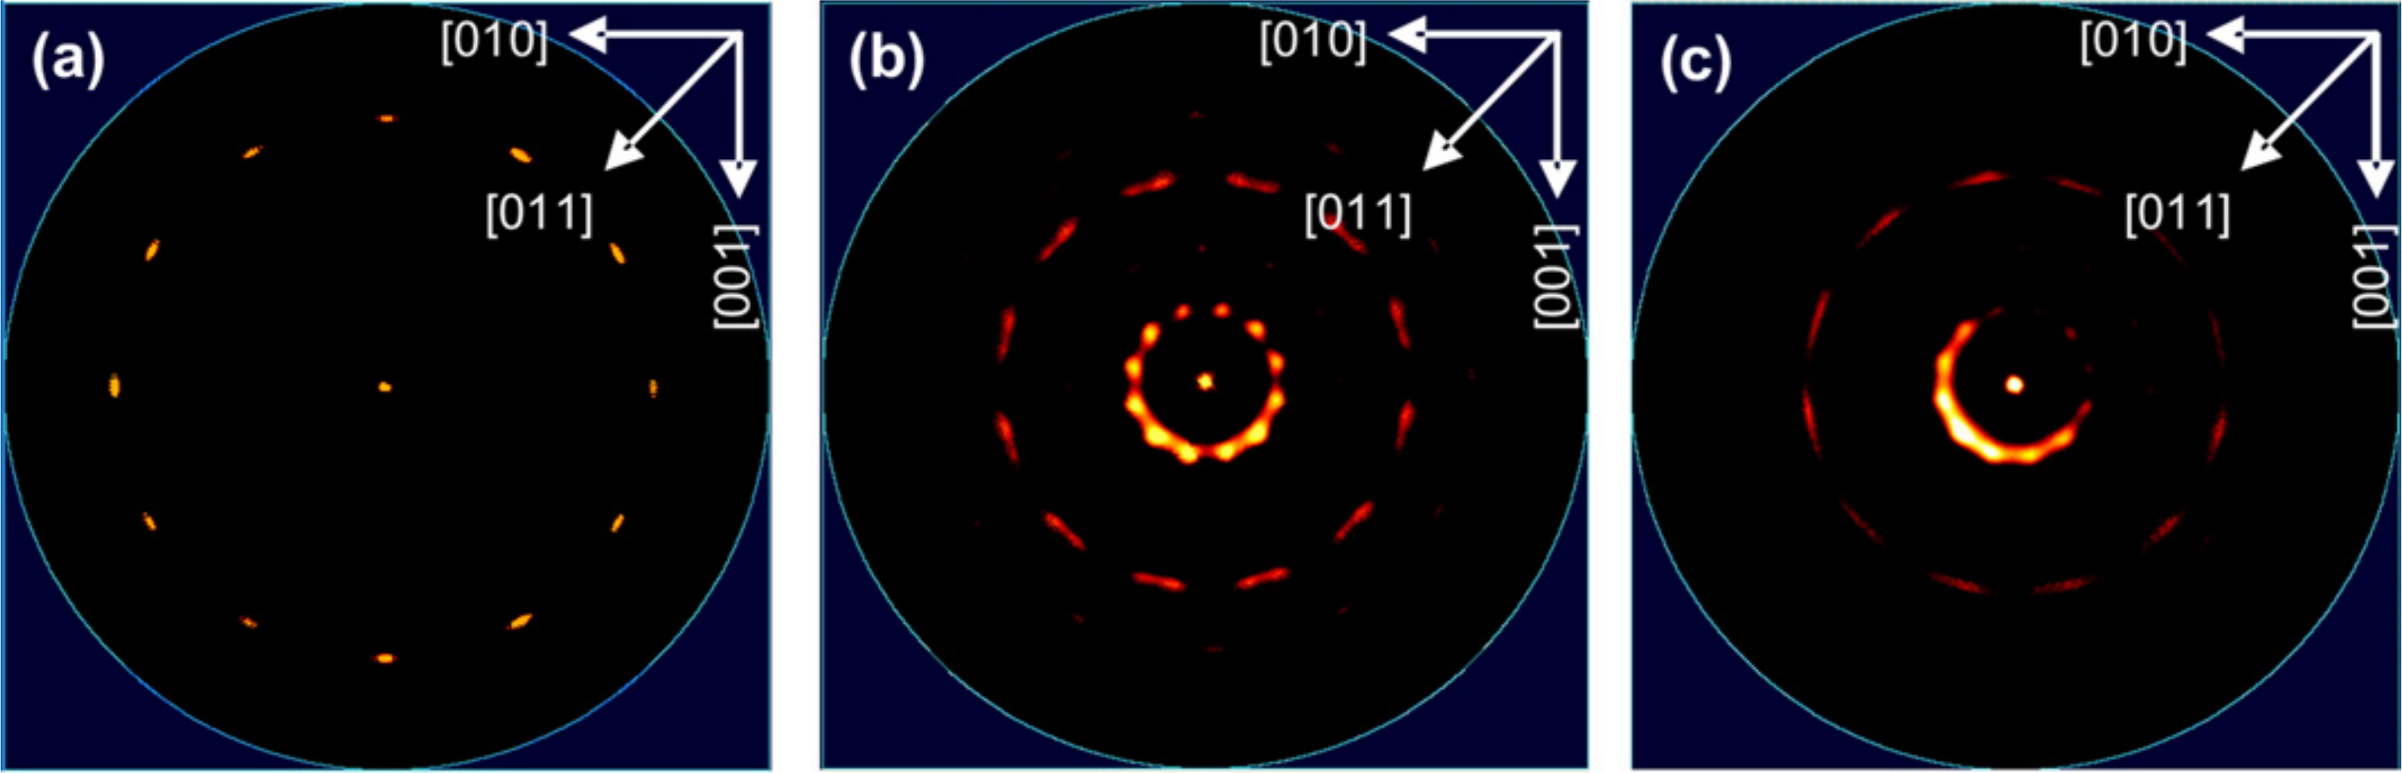
\includegraphics[width=\textwidth]{srtio3_pole}
    \caption{\label{fig:srtio3_pole}(1 1 1) CdTe pole figures for films deposited on (a) the as-received (1 0 0) SrTiO3 substrate (b) the reconstructed surface with wide terraces and (c) the reconstructed
        surface with narrow terraces. Indicated on each image are the substrate’s in-plane crystallographic axes obtained from XRD measurements.}
\end{figure}



\section{Implications for Symmetry and Energy at Epitaxial Surfaces}